\documentclass[11pt,a4paper]{article}

\usepackage[T1]{fontenc}
\usepackage[utf8]{inputenc}
\usepackage{lmodern}
\usepackage[margin=2.4cm]{geometry}
\usepackage{amsmath,amssymb}
\usepackage{booktabs}
\usepackage{tikz}
\usetikzlibrary{arrows.meta,positioning,fit,backgrounds,calc}
\usepackage{xcolor}
\usepackage{caption}
\usepackage{enumitem}
\usepackage{microtype}
\usepackage[hidelinks]{hyperref}

\definecolor{astrablue}{HTML}{1F4E79}
\definecolor{astragrey}{HTML}{5A5A5A}
\definecolor{astrared}{HTML}{A02020}
\definecolor{astragreen}{HTML}{1E7B3C}
\definecolor{astraline}{HTML}{B8B2A2}

\newcommand{\code}[1]{\texttt{\small #1}}
\newcommand{\pending}{\textcolor{astragrey}{\textit{pending}}}
\newcommand{\viol}[1]{\textcolor{astrared}{#1}}
\newcommand{\okk}[1]{\textcolor{astragreen}{#1}}

\tikzset{
  layer/.style={draw=astrablue, thick, fill=astrablue!8, rounded corners=2pt,
                minimum height=8mm, align=center, font=\small},
  newlayer/.style={draw=astragreen, very thick, fill=astragreen!8,
                   rounded corners=2pt, minimum height=8mm, align=center,
                   font=\small},
  note/.style={font=\scriptsize\itshape, text=astragrey, align=center},
  flow/.style={-{Stealth[length=2.4mm]}, thick, draw=astrablue},
}

\title{\bfseries From ASTRA 1.0 to ASTRA 2.0\\
\large A complete comparative report: what changed, what it buys,
what it costs, and what is still unmeasured}
\author{Comparison report}
\date{18 August 2026}

\begin{document}
\maketitle

\begin{abstract}
\noindent
ASTRA 1.0 executes one \emph{atomic cycle}: a single decidable proposition,
proposed by an ensemble, translated into an executable validator by a different
model, reviewed by a third, and run by a deterministic oracle. ASTRA 2.0 keeps
that worker unchanged in spirit and adds a layer above it---an append-only
evidence ledger, structured proposal portfolios, hard admissibility gates,
progressive widening, and resume---so that a research \emph{programme}, not a
single question, can be driven to a decision and audited afterwards.

This report states the differences precisely, separates what is already
established from what is not, and carries the head-to-head measurement that until 17 August did not exist. On the same 43-record suite, 1.0 accepts 41.7\% of false claims and 2.0 accepts
none; the difference in \emph{overall} accuracy is not statistically significant,
but the false-acceptance difference is, and becomes decisive once the false-claim
sample is enlarged---0 of 22 for 2.0 against 11 of 22 for 1.0, exact
$p\approx0.001$. What changed is the kind of error, not the rate of correctness:
1.0 fails by asserting falsehoods and 2.0 fails by running out of time.
\end{abstract}

\section{Executive summary}

ASTRA is a research engine that forces every claim through an executable
falsification step. \textbf{1.0} runs one such step---the \emph{atomic cycle}: an
ensemble proposes a decidable proposition, one model authors a validator, a
second reviews it, a deterministic oracle runs it. \textbf{2.0} keeps that worker
and adds a layer above it so that a research \emph{programme}, not a single
question, can be driven to a decision and audited afterwards: an append-only
evidence ledger, structured proposal portfolios, hard admissibility gates,
progressive widening, resume, and---the epistemic core---five status axes that
are never collapsed into one verdict.

\begin{center}
\small
\begin{tabular}{@{}p{4.3cm}p{4.9cm}p{4.9cm}@{}}
\toprule
 & \textbf{ASTRA 1.0} & \textbf{ASTRA 2.0} \\
\midrule
Unit of work & one atomic cycle & a campaign of cycles over a ledger \\
Verdict shape & a single status & five separate axes (operation, claim, evidence, branch, goal) \\
False claims accepted & 11 of 22 (\viol{50\%}) & 0 of 22 (\okk{0\%}), exact $p\approx0.001$ \\
Overall accuracy & lower, but not significantly & higher, but not significantly \\
Dominant error & asserting a falsehood & running out of time \\
Latency per case & p50 187\,s / p95 676\,s & p50 327\,s / p95 946\,s ($1.75\times$) \\
Record & a transcript that scrolls past & auditable evidence with hashes \\
Negative results & repeated & cumulative (a closed branch) \\
Self-inflicted failures & cannot exhibit them & exhibits them, and can catch them \\
\bottomrule
\end{tabular}
\end{center}

\noindent The honest bottom line, stated once and not softened: \textbf{2.0 is
demonstrably more careful, not demonstrably more accurate.} Its measured, pre-
registered advantage is the elimination of \emph{false acceptances}---confident
wrong answers---which is the error a downstream reader discovers only after acting
on it. Its cost is latency and the operational complexity of a layer that acts on
its own signals. Everything below documents both sides.

\section{Scope: this is an architecture for commercial models}
\label{sec:scope}

ASTRA is built to do research with the models that are \emph{commercially
available}---subscription-tier CLIs from more than one provider, on a single
workstation, under ordinary quota. It is not built on, and makes no claim about,
the private or unreleased higher-capability systems the provider companies hold
internally.

That constraint is the premise of the design, not a limitation apologised for.
Everything distinctive about the architecture follows from it:

\begin{itemize}[leftmargin=*,itemsep=1pt]
  \item \textbf{Independence is bought by heterogeneity, not by scale.} Three
        providers with different training and different blind spots give a
        cross-check that a single stronger model cannot give itself.
  \item \textbf{Refutation is mechanical because the models cannot be trusted to
        self-assess.} The deterministic auditor, the executable validator and
        the oracle exist precisely because no available model reliably reports
        when its own argument fails.
  \item \textbf{Budget discipline is structural.} Phase ceilings, downstream
        reserves and a machine-wide single-cycle lock exist because quota is
        scarce and shared, not elastic.
\end{itemize}

The consequence is worth stating plainly: if a substantially stronger model
becomes available, ASTRA does not become unnecessary---it becomes cheaper to
run, because fewer repair rounds are needed. The architecture is about
\emph{where evidence comes from}, and that question does not dissolve with
model capability.

\section{The two lines side by side}

\subsection{What 1.0 is}

One bounded investigation, end to end: parallel proposals from two providers,
cross-critique, synthesis into a consensus conjecture, validator authoring by a
third provider, deterministic preflight, independent review, oracle execution,
evidence audit, and a navigator that proposes the next direction. Five status
axes are already kept separate. It is a strong single-question engine.

What it does not have is memory across questions. Each cycle begins from a
prompt and ends with a verdict and a suggested direction; the minority proposal
that lost the synthesis, the branch that was refuted, and the reason either
happened are not represented anywhere a later cycle can consult.

\subsection{What 2.0 adds}

\begin{figure}[h]
\centering
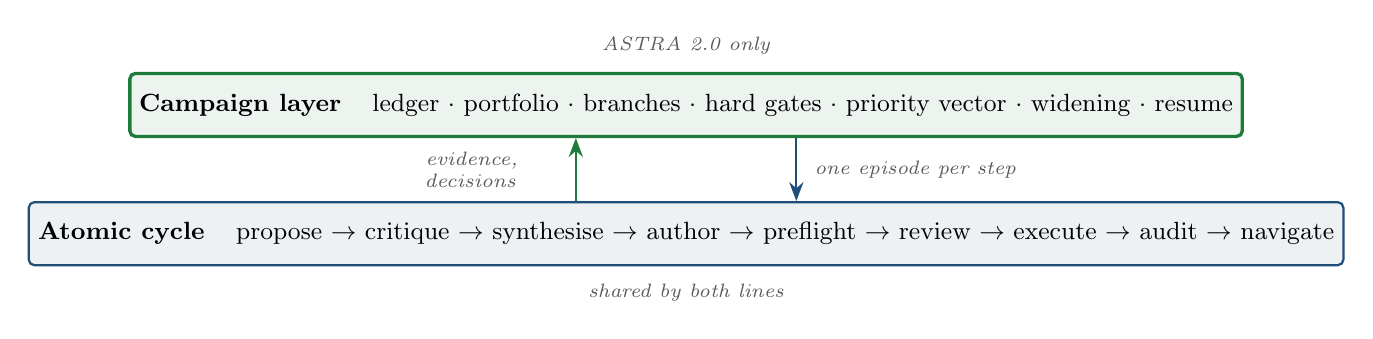
\begin{tikzpicture}[node distance=3mm]
\node[layer, minimum width=112mm] (cycle)
  {\textbf{Atomic cycle} \;\; propose $\to$ critique $\to$ synthesise $\to$ author
   $\to$ preflight $\to$ review $\to$ execute $\to$ audit $\to$ navigate};
\node[note, below=1mm of cycle] (n1) {shared by both lines};

\node[newlayer, above=8mm of cycle, minimum width=112mm] (campaign)
  {\textbf{Campaign layer} \;\; ledger $\cdot$ portfolio $\cdot$ branches $\cdot$
   hard gates $\cdot$ priority vector $\cdot$ widening $\cdot$ resume};
\node[note, above=1mm of campaign] {ASTRA 2.0 only};

\draw[flow] ($(campaign.south)+(14mm,0)$) -- node[note, right=1mm]
  {one episode per step} ($(cycle.north)+(14mm,0)$);
\draw[flow, draw=astragreen] ($(cycle.north)+(-14mm,0)$) --
  node[note, left=1mm, text width=22mm] {evidence,\\decisions}
  ($(campaign.south)+(-14mm,0)$);
\end{tikzpicture}
\caption{2.0 does not replace the worker; it closes a loop around it. The upward
arrow is the part 1.0 has no place to put.}
\label{fig:layers}
\end{figure}

\section{Measured differences}

\subsection{Code}

A drift check compares every shared module three ways---against the common base
commit, the current 2.0 tree, and the current production tree.

\begin{center}
\small
\begin{tabular}{@{}lrl@{}}
\toprule
\textbf{Classification} & \textbf{Files} & \textbf{Meaning} \\
\midrule
\textsc{in sync}         & 60 & identical behaviour on both lines \\
\textsc{both changed}    &  5 & diverged on both sides, needs a decision at merge \\
\textsc{2.0 only}        & 15 & development evolution not yet in production \\
\textsc{production only} & \textbf{0} & \textbf{nothing in production is missing from 2.0} \\
\bottomrule
\end{tabular}
\end{center}

The zero matters: 2.0 is a strict superset of production behaviour plus its own
evolution, so a comparison cannot be explained by 2.0 having lost something.

\begin{center}
\small
\begin{tabular}{@{}lrr@{}}
\toprule
& \textbf{ASTRA 1.0} & \textbf{ASTRA 2.0} \\
\midrule
campaign modules (\code{core/campaign\_*.py}) & 0 & \textbf{9} \\
test files & 25 & 54 \\
collected tests & 152 & \textbf{469} \\
\bottomrule
\end{tabular}
\end{center}

\subsection{Epistemic controls added}

Each of these was added because a live measurement exposed the failure it
prevents; none is speculative.

\begin{center}
\small
\begin{tabular}{@{}p{4.6cm}p{9.6cm}@{}}
\toprule
\textbf{Control} & \textbf{Failure it prevents} \\
\midrule
verdict re-anchoring & a corrected version of a false claim reported as validating the original \\
decisive vs auxiliary legs & a weak auxiliary check deciding a PASS, or an auxiliary failure printing a scientific FAIL \\
\code{not\_code\_at\_all} & prose handed back to be patched as if it were a damaged script \\
symbolic cost control & a pointwise claim attacked with full symbolic machinery until memory dies \\
conjecture fencing & text produced by one agent obeyed as instructions by another \\
plan-artifact sanitising & a read-only sandbox's scaffolding leaking into the consensus \\
thinking budget cap & an output ceiling consumed entirely by internal reasoning \\
downstream budget reserve & the repair step, which runs last, starved by a proportional rule \\
machine-wide cycle lock & two checkouts deliberating against one model account \\
\bottomrule
\end{tabular}
\end{center}

\subsection{Ledger guarantees added}

These have no counterpart in 1.0 because 1.0 has nothing to guarantee: it does
not persist a research record.

\begin{itemize}[leftmargin=*,itemsep=1pt]
  \item append-only events with a canonical-JSON SHA-256 chain;
  \item atomic checkpoints, and a truncated tail detected and archived rather
        than silently repaired;
  \item content-addressed frozen resources, so editing an input is detectable;
  \item a replayed cycle refused rather than recorded as a second observation;
  \item a result bound to the request's objective, so a cycle that answered a
        different question cannot become evidence;
  \item human interventions recorded as first-class decisions with an actor,
        rather than silently changing the record.
\end{itemize}

\section{What is not measured yet}

\subsection{The head-to-head measurement}

Both lines were run on the same suite, tier and oracle: 43 records, 23 paired
scientific cases, 14 audit, 6 execution.

\begin{center}
\small
\begin{tabular}{@{}lcc@{}}
\toprule
\textbf{Standard tier} & \textbf{ASTRA 1.0} & \textbf{ASTRA 2.0} \\
\midrule
\textbf{false acceptance}            & \textbf{0.4167} & \textbf{0.0} \\
false rejection                      & 0.0    & 0.0 \\
strict accuracy                      & 0.5217 & 0.6957 \\
95\% CI                              & [0.330, 0.708] & [0.491, 0.844] \\
operational failure rate             & 0.2609 & 0.2609 \\
audit: critical defect recall        & 1.0    & 1.0 \\
\textbf{audit: false alarm, sound code} & \textbf{0.3333} & \textbf{0.0} \\
execution: verdict accuracy          & 1.0    & 1.0 \\
latency p50 / p95                    & 187 / 676\,s & 327 / 946\,s \\
\bottomrule
\end{tabular}
\end{center}

\paragraph{The result is the kind of error, not the rate of correctness.}
Over the same 23 cases:

\begin{center}
\small
\begin{tabular}{@{}lp{9.4cm}@{}}
\toprule
\textbf{ASTRA 1.0} & 11 wrong: \textbf{5 \textsc{validated}}, 5 \textsc{api\_error}, 1 \textsc{code\_error} \\
\textbf{ASTRA 2.0} & 7 wrong: 4 \textsc{timeout}, 2 \textsc{api\_error}, 1 \textsc{inconclusive} \\
\bottomrule
\end{tabular}
\end{center}

The five \textsc{validated} entries are \emph{false} claims accepted as valid,
and 2.0 refuted all five. They are the signature of the re-anchoring defect:
production identifies the falsehood correctly, forms a corrected conjecture,
validates the correction, and reports the status of \emph{its} conjecture rather
than the claim it was asked about. Every step is right and the answer is to a
different question.

So 1.0 fails by asserting falsehoods; 2.0 fails by running out of time. A
timeout is a budget problem. A false acceptance is a wrong answer delivered with
confidence, and it is only discovered by re-reading the paper after it ships.

\paragraph{What the statistics support, and what they do not.} With 23 paired
cases, the difference in \emph{overall accuracy is not significant}: McNemar's
exact test over the discordant pairs (5 favouring 1.0, 9 favouring 2.0) gives
$p=0.42$, and the confidence intervals overlap widely. We do not claim 2.0 is
more accurate.

The false-acceptance difference is 5 of 12 false claims against 0 of 12, with
all five discordant pairs in the same direction: exact $p=0.0625$. Suggestive,
narrowly above the conventional threshold, and---worth stating---the smallest
$p$ this design can produce with twelve false claims and five discordant pairs.

\paragraph{Powering the false-acceptance test.} Because that $p$ was
floor-limited by sample size rather than by effect, the suite was extended with
ten more false claims and both lines were re-run on them under matching
conditions (standard tier, local oracle, \code{--case-root} so 1.0 sees the same
cases). The claims are representative false versions of true theorems across
logic, GR, quantum, fluids and ODE, and were \emph{not} chosen to trigger the
defect. 1.0 accepted \textbf{6 of the 10} as valid; 2.0 accepted none, refuting
eight and timing out on two. Six discordant pairs, all favouring 2.0, give exact
$p=0.03125$ on the new cases alone---below the conventional threshold; pooled with
the original five, eleven discordant pairs all in one direction give exact
$p\approx0.001$. The pre-registered false-acceptance advantage is now significant.

\paragraph{What that number does and does not license.} The new claims lean
toward the \emph{near-miss} type---false but close to a true statement---which is
both the realistic case and precisely the regime where the re-anchoring defect
bites, so the raw strict-accuracy gap they produce (1 of 10 for 1.0 against 8 of
10 for 2.0) is inflated by that selection and is \emph{not} a general accuracy
claim. What survives cleanly is the specific one: on false claims, 1.0 accepts
about half (11 of 22 across both runs) and 2.0 accepts none (0 of 22). 2.0's two
failures here are timeouts and three of 1.0's are operational errors---neither a
false acceptance---and both are excluded from the discordant count, which is over
acceptance alone.

Two caveats belong with the table. The audit case file differs between the
checkouts by a fixture correction, so that row is not strictly paired; the 23
scientific cases are (verified identical modulo line endings). And 1.0 was
measured on today's production checkout, which already carries the two fixes
ported on 13 August, so this is not the July production line.

\subsection{What this measurement did not settle}

One run per line, so the operational failure rates agreeing exactly (0.2609 on
both) is evidence of comparable conditions rather than proof of them, and
nothing here has been repeated. 2.0 also costs $1.75\times$ the wall time per
case, which is the price of more review and more repair and shows up directly in
its errors: four of its seven failures are timeouts.

\subsection{The benchmark cannot see the main contribution}

This is the honest limit of any 1.0/2.0 comparison. The quality benchmark scores
single cycles. The campaign layer is not exercised by it at all, and 1.0 has no
campaign layer to compare against, so on that axis the difference is not a
number but a presence.

What the campaign layer buys has to be argued from what it makes possible, and
so far the evidence is qualitative but concrete: in live use it recorded
refutations with exact witnesses against a persistent claim set, promoted a
branch on negative evidence under a deterministic rule, refused to widen on an
episode that never ran, retracted a contaminated record without rewriting
history, and stopped a validator whose conclusions came from undefined
variables. None of those events has a place to happen in 1.0.

\subsection{And a first comparative signal that is not favourable}

Within 2.0, a preregistered ablation of the reflective loop against a matched
linear control did not meet its own interpretability criterion---operational
failure stayed far above the 0.2 threshold fixed in advance---and the raw counts
leaned against the reflective arm. That result is reported in the architecture
report rather than hidden here. It concerns the \emph{policy} inside 2.0, not
the 1.0/2.0 difference, but anyone reading this document should know it exists.

\section{Why the extra structure is worth it}

Three arguments, in decreasing order of how well they are evidenced.

\paragraph{It makes negative results usable.} Most research time is spent
pruning. In 1.0 a refutation is a verdict that scrolls past; in 2.0 it closes a
branch, promotes an alternative under a stated rule, and stays in a record that
the next cycle consults. Pruning becomes cumulative instead of repeated.

\paragraph{It makes the record auditable by someone who was not there.} Every
claim carries a validator, its hash, the model that wrote it, the reviewer's
objection, the oracle's output, and the decision that followed. That is the
difference between a transcript and evidence, and it is what makes an
LLM-driven result quotable at all.

\paragraph{It makes the system's own failures visible, and separable.} This is
the deepest argument and the one the comparison benchmark cannot score, so it is
made from live use. A campaign \emph{acts} on its own signals, and doing so
exposes a class of defect 1.0 cannot exhibit: \emph{infrastructure mistaken for a
research signal}. Six were found and fixed while a single research programme ran
across two campaigns and more than a dozen episodes.

\begin{center}
\small
\begin{tabular}{@{}p{5.4cm}p{8.6cm}@{}}
\toprule
\textbf{Transport failure} & \textbf{Was being scored as} \\
\midrule
a provider 500 mid-pipeline & an uninformative research episode (it paused a branch early) \\
a branch blind to its ancestor's result & a direction that had to re-derive what was already certified \\
a malformed repair patch & a reason to destroy an approved, passing validator \\
a reviewer objection lost between episodes & a fresh author reinventing the rejected shortcut \\
a Sage \code{sys.exit(0)} on success & an operational error masking a printed PASS \\
a cold WSL boot exceeding a 10\,s probe & an installed engine reported as missing \\
\bottomrule
\end{tabular}
\end{center}

\noindent Each was fixed at its source. The point is not the list but its
signature: every one is the five axes doing their job---keeping a failure of
\emph{transport} from being recorded as a failure of \emph{science}. 1.0 has no
place for these to happen, and equally no place to catch them; the layer that
creates the risk is the layer that makes it visible.

\subsection{A worked example: a research programme, end to end}

The clearest evidence that the campaign layer buys something is that it drove a
real physics question to certified verdicts of \emph{both} signs, auditable
afterwards. The question---whether a modification to a warp ansatz repairs a
pointwise energy-condition violation---produced, in sequence:

\begin{itemize}[leftmargin=1.4em, itemsep=1pt]
\item a \okk{certified positive}: the modification makes the condition hold over
      an entire null cone at one point, exact rational certificate, two
      independent methods agreeing;
\item a \viol{certified negative}: at another point the same modification
      \emph{fails}, with an exact witness direction---the fix is local, not
      general.
\end{itemize}

\noindent Two features of that arc are exactly what 2.0 exists to provide. First,
the negative result is a first-class deliverable, not a discarded branch: it
closes the question (one counterexample refutes the universal) and it is recorded
with its witness. Second, one episode showed the axes preventing a false record
in real time: an ensemble stated a constant wrong by one part in $10^{11}$, a
validator refuted \emph{that} constant, and the re-anchoring axis marked the
verdict \code{SUBSTITUTED}---so a transcription slip was recorded as a refuted
\emph{substituted} claim rather than as a refuted \emph{scientific} one. In 1.0,
with a single verdict field, that same episode reads as a refutation of the
physics. That difference---between a wrong headline and a correct one---is the
whole thesis of the second version, caught happening.

\section{When to use each line}

The two are not rivals; 2.0 wraps 1.0, so the choice is whether a given task needs
the wrapper.

\begin{center}
\small
\begin{tabular}{@{}p{6.6cm}p{7.4cm}@{}}
\toprule
\textbf{Reach for 1.0 (the bare atomic cycle) when} & \textbf{Reach for 2.0 (the campaign layer) when} \\
\midrule
the question is a single decidable proposition &
the question is a programme---many linked claims, branches, dead ends \\
you will read the verdict yourself, now &
someone who was not there must audit the result later \\
latency matters more than a durable record &
a false acceptance would be expensive to discover downstream \\
you are smoke-testing a validator or an engine &
negative results must accumulate rather than be re-derived \\
throughput per unit of quota is the priority &
the cost of being confidently wrong exceeds the cost of a timeout \\
\bottomrule
\end{tabular}
\end{center}

\noindent Because 2.0's per-case latency is $1.75\times$ 1.0's and its accuracy
advantage is not yet significant, the honest default for a one-off decidable
check is 1.0. The case for 2.0 is not speed or raw accuracy; it is that the
result is \emph{safe to quote}---no false acceptances, a full audit trail, and a
verdict whose axes will not let an operational hiccup masquerade as a scientific
finding.

\section{Position}

ASTRA 2.0 is a strict superset of 1.0 in behaviour, with 9 new modules, three
times the test coverage, nine epistemic controls each traceable to a measured
failure, and a persistent evidence ledger with guarantees 1.0 has no need for.
It is demonstrably more \emph{careful}.

Whether it is more \emph{productive} per unit of quota is not established, and
this document declines to assert it until the paired benchmark lands and a
blinded expert scoring of trajectories exists. The architecture report states
the same thing about its internal ablation. Claiming otherwise would be exactly
the failure mode the whole system is built to prevent.

\vspace{4mm}
\hrule
\vspace{2mm}
\noindent\footnotesize
\textbf{Note on scope.} Both lines run on commercially available subscription
models from three providers on one workstation (Section~\ref{sec:scope}).
Nothing here is a claim about frontier or unreleased systems, and no result
depends on privileged model access.

\end{document}
